\begin{figure}[htbp]
\centering
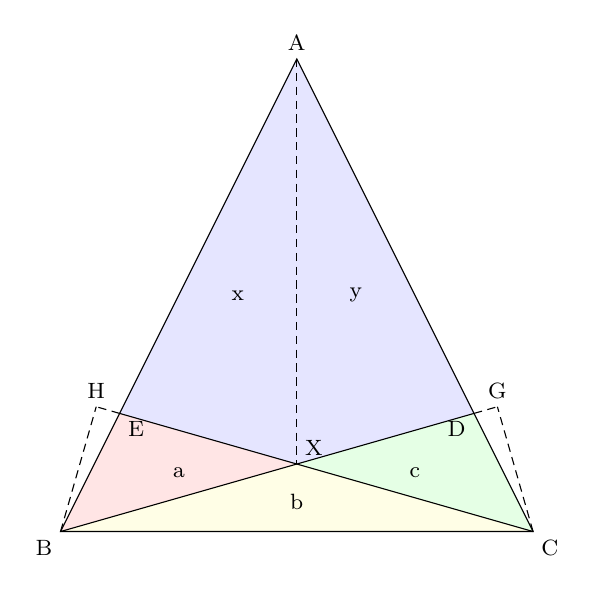
\begin{tikzpicture}[scale=1.5]
\footnotesize
\coordinate (A) at (2,4);
\coordinate (B) at (0,0);
\coordinate (C) at (4,0);
\coordinate (D) at (3.5, 1);
\coordinate (E) at (0.5, 1);
\coordinate (H) at (16/53, 56/53);
\coordinate (G) at (4-16/53, 56/53);
\coordinate (X) at (2, 4/7);

\filldraw[draw=none,fill=red!10] (B) -- (E) -- (X) -- cycle;
\filldraw[draw=none,fill=green!10] (C) -- (D) -- (X) -- cycle;
\filldraw[draw=none,fill=yellow!10] (B) -- (C) -- (X) -- cycle;
\filldraw[draw=none,fill=blue!10] (A) -- (E) -- (X) -- (D) -- cycle;

\node[above] at (A) {A};
\node[below left] at (B) {B};
\node[below right] at (C) {C};
\node[below left] at (D) {D};
\node[below right] at (E) {E};
\node[above] at (H) {H};
\node[above] at (G) {G};
\node[above right] at (X) {X};

\node at (2, 0.25) {b};
\node at (1, 0.5) {a};
\node at (3, 0.5) {c};
\node at (1.5, 2) {x};
\node at (2.5, 2) {y};

% AB: y = 2x; AC: -2x + 8
% BD: y = 2x/7; CE; -2x/7 + 8/7
\draw (A) -- (B) -- (C) -- cycle;
\draw (B) -- (D);
\draw (C) -- (E);

% BH: 7x/2
\draw[densely dashed] (B) -- (H);
\draw[densely dashed] (E) -- (H);
\draw[densely dashed] (C) -- (G);
\draw[densely dashed] (D) -- (G);
\draw[densely dashed] (A) -- (X);

\end{tikzpicture}
\end{figure}
